\documentclass{beamer}

\usepackage{graphicx,hyperref,udesc,url}
\usepackage[utf8]{inputenc}
\usepackage[T1]{fontenc}
\usepackage{booktabs}
%\usepackage[portugues]{babel}
\usepackage{amssymb}
\usepackage[utf8]{inputenc}
\usepackage[brazil]{babel}
\usepackage{csquotes}
\usepackage{listings}
\usepackage{amsmath}
\usepackage{amsthm}
\usepackage{mathtools}
\usepackage{verbatim}
%\usepackage[table,xcdraw]{xcolor}
\usepackage{multirow}

\title[]{Otimizações para Motores de Jogos Através de Modelagem Orientada a Dados}

\author[Vinicius Bruch Zuchi]{
    Vinicius Bruch Zuchi\\\medskip
    {\small \url{vinicius.b.zuchi@gmail.com}\\}}

\institute[UDESC]{
    Departamento de Ci\^encia da Computa\c{c}\~ao \\
    Centro de Ci\^encias e Tecnol\'ogicas\\
Universidade do Estado de Santa Catarina}

\begin{document}

\begin{frame}
    \titlepage
\end{frame}

\begin{frame}
    \frametitle{Sum\'ario}
    \tableofcontents
\end{frame}

\section{Motivação}

\frame{\tableofcontents[currentsection]}

\begin{frame}[t]{Otimizações}
    \par\medskip
    \vspace{1.5cm}
    '' We should forget about small efficiencies, say about 97\% of the time: premature 
    optimization is the root of all evil. Yet we should not pass up our opportunities in 
    that critical 3\% `` \\ - Donald Knuth, 1974
\end{frame}

\begin{frame}[t]{Hierarquia de Memória}
    \begin{figure}
        \centering
        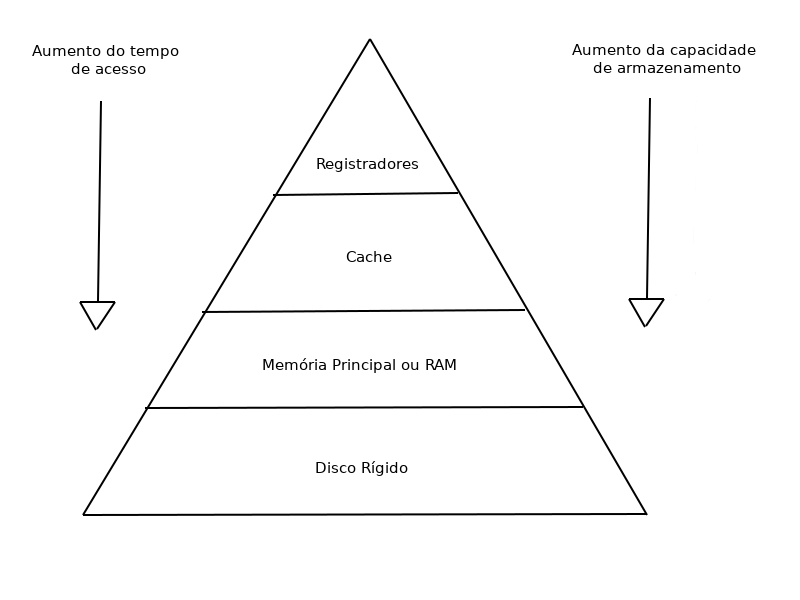
\includegraphics[width=.8\textwidth]{figuras/memoryhierarchy}
    \end{figure}
\end{frame}

\begin{frame}[t]{O Gargalo de Desempenho}
    \begin{itemize}
        \item Acesso à memória é o real gargalo de desempenho
        \item CPU's atualmente são extremamente rápidos
        \item A memória é muito lenta quando comparada ao CPU
    \end{itemize}
\end{frame}

\begin{frame}[t]{O Gargalo de Desempenho}
    \begin{itemize}
        \item Tecnologia da memória não evoluiu com a mesma velocidade que a tecnologia 
            do CPU
        \begin{itemize}
            \item De 1986 até agora a velocidade do CPU aumentou cerca de 55\% a 60\% 
                por ano
            \item Velocidade da memória aumentou apenas 10\% por ano
        \end{itemize}
        \item Ao realizar uma operação e os dados necessários não estão no cache:
            \begin{itemize}
                \item Cache miss
                \item CPU permanece ocioso por vários ciclos até esperar os dados 
                    chegarem
            \end{itemize}
    \end{itemize}
\end{frame}

\begin{frame}[t]{O Quão Ruim É?}
    \vspace{1.5cm}
    \begin{itemize}
        \item Para pegar uma linha de cache (64 bit)
            \begin{itemize}
                \item DDR3 SDRAM (1333 MHz) \~{} 11 nanosegundos
            \end{itemize}
        \item Intel Core i7
            \begin{itemize}
                \item 117 160 MIPS \~{} 117 instruções por nanosegundo
            \end{itemize}
        \item 1287 ciclos de CPU gastos por cache miss completo
    \end{itemize}
\end{frame}

\section{Modelagem Orientada a Dados}

\frame{\tableofcontents[currentsection]}

%\frame{\tableofcontents
    %[
        %currentsection,
        %currentsubsection,
        %subsectionstyle=show/shaded/hide
    %] }

\begin{frame}[t]{Modelagem Orientada a Dados}
    \begin{itemize}
        \item Introduzida por John A. Sharp em 1980
        \item Seu objetivo era aprimorar o tempo de processamento e eficiência da 
            memória
        \item Dados são o foco, e são representados por \textit{arrays} armazenados na 
            memória de forma contígua
        \item Leitura sequencial dos dados
        \item Separação dos dados "quentes"\ e "frios"
    \end{itemize}
\end{frame}

\begin{frame}[t]{Diferença de MOO e MOD}
    \begin{figure}
    \centering
        \begin{minipage}[b]{0.35\textwidth}
            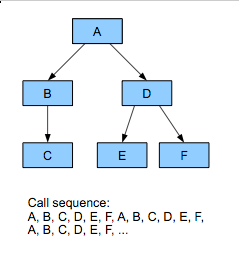
\includegraphics[width=\textwidth]{figuras/objectreadingorder}
        \end{minipage}
        \begin{minipage}[b]{0.35\textwidth}
            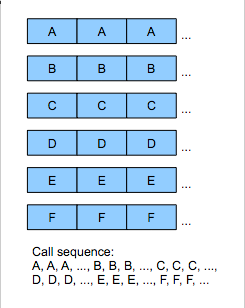
\includegraphics[width=\textwidth]{figuras/dodreadingorder}
        \end{minipage}
        %\par\medskip
        %Disponível em: <http://gamesfromwithin.com/data-oriented-design>. Acesso em: 27/05/2017.
        %\label{oodvsdod}
    \end{figure}
\end{frame}

\begin{frame}[t]{Vantagens e Desvantagens da MOO}
    \begin{minipage}[b]{0.4\textwidth}
        Vantagens da MOO
        \begin{itemize}
            \item Modular - objetos são independentes
            \item Black-box
            \item Conceitual - mapeamento com o mundo real
            \item Reutilizável
        \end{itemize}
    \end{minipage}
    \hspace{1.5cm}
    \begin{minipage}[b]{0.4\textwidth}
        Desvantagens da MOO
        \begin{itemize}
            \item Pior desempenho - prejudicial ao cache
            \item Ênfase no design, promove engenharia em excesso
            \item Difícil de separar em threads
        \end{itemize}
    \end{minipage}
\end{frame}

\begin{frame}[t]{Vantagens e Desvantagens da MOD}
    \begin{minipage}[b]{0.4\textwidth}
        Vantagens da MOD
        \begin{itemize}
            \item Simples e modular
            \item Melhor utilização do cache e desempenho (blocos homogêneos sequenciais)
            \item Melhor paralelização - fácil mover e transformar dados entre múltiplas 
                threads ou núcleos
        \end{itemize}
    \end{minipage}
    \hspace{1.5cm}
    \begin{minipage}[b]{0.4\textwidth}
        Desvantagens da MOD
        \begin{itemize}
            \item Conceito difícil de entender - requer uma maneira diferente de 
                raciocínio
            \item Difícil de integrar com POO
            \item Código com menos abstração
        \end{itemize}
    \end{minipage}
\end{frame}

\section{Rust}

\frame{\tableofcontents[currentsection]}

\begin{frame}[t]{Linguagem de Programação Rust}
    \begin{itemize}
        \item Desenvolvida pela Mozilla
        \item Primeiro release em 2015
        \item Linguagem de sistemas de propósito geral e multiparadigma
        \item Influências de linguagens imperativas e funcionais
    \end{itemize}    
\end{frame}

\begin{frame}[t]{Características da Linguagem}
    %*Falar sobre velocidade, segurança de memória, abstrações sem custo, e comparável 
    %ao C e C++*
    \begin{itemize}
        \item Tem como objetivos segurança, velocidade e concorrência
        \item Não utiliza garbage collector
        \item Controle completo do layout da memória
        \item Abstrações sem custo e posse (ownership system)
        \item Equiparável ao C++, porém mais seguro em termos de memória
    \end{itemize}    
\end{frame}

\section{Motor de Jogos}

\frame{\tableofcontents[currentsection]}

\begin{frame}[t]{Conceito}
    \begin{itemize}
        \item Separação entre a parte técnica e a parte criativa do jogo
        \item Vários componentes integrados, cada um responsável por uma parte diferente
        \item Integração dos componentes forma a arquitetura do motor e os loops do jogo
    \end{itemize}
\end{frame}

\begin{frame}[t]{Motor de Jogos}
    \begin{itemize}
        \item Modularização, rápida prototipagem e desenvolvimento, e portabilidade 
            dos jogos
        \item Foi rapidamente adotado pela indústria de jogos desde seu surgimento
        \item Um motor de jogos bem estruturado facilita o desenvolvimento de um jogo 
            eficiente
    \end{itemize}
\end{frame}

\begin{frame}[t]{MOD e Jogos}
    %*Explicar que tem muitas variáveis e entidades, precisam ser constantemente 
    %atualizadas, muitos objetos com muitos dados fracamente relacionados, 
    %poluição do cache*
    \begin{itemize}
        \item Muitas dados e entidades
        \item Necessitam constante atualização e processamento
        \item MOO pode gerar classes com muitos atributos fracamente relacionados
        \item Poluição do cache
        \item Processamento sequencial dos dados é desejável
    \end{itemize}
\end{frame}

\section{Trabalhos Relacionados}

\frame{\tableofcontents[currentsection]}

\begin{frame}[t]{Trabalhos Relacionados}
    \begin{itemize}
        \item Nenhuma proposta diretamente relacionada encontrada
        \item O conceito de MOD voltou a ser discutido apenas recentemente
        \item Mais difundido entre a comunidade de desenvolvedores de jogos
        \item Dois artigos explicitamente falando sobre MOD
    \end{itemize}
\end{frame}

\section{Proposta de Trabalho}

\frame{\tableofcontents[currentsection]}

\begin{frame}[t]{Motor de Jogos com MOD}
    %*Explicar que vou usar uma engine como caso de estudo, vou explorar o potencial da 
    %MOD e do Rust, depois vou fazer análise e comparar com POO*
    \begin{itemize}
        \item Implementação de um motor de jogos com os conceitos de CG
        \item Elaboração da sua arquitetura e módulos utilizando a MOD
        \item Desenvolvimento de uma aplicação utilizando o motor e também a MOD
        \item Análise e comparação do trabalho desenvolvido com uma abordagem que 
            utilize a POO
    \end{itemize}
\end{frame}

\section{Conclusões Parciais e Próximas Etapas}

\frame{\tableofcontents[currentsection]}

\begin{frame}[t]{Conclusões Parciais}
    \begin{itemize}
        \item Jogos lidam com muitos dados simultaneamente e partes críticas do código 
            precisam de otimizações
        \item Devido a essa quantidade de dados e ao gargalo de desempenho da memória, 
            seus códigos precisam ser estruturados de uma maneira coerente com a 
            arquitetura da memória
        \item Encontrou-se uma maneira de otimizar o código além da paralelização, a 
            Modelagem Orientada a Dados
        \item Pouco material na literatura sobre MOD e Rust, surge então uma boa 
            oportunidade para explorá-los
    \end{itemize}
\end{frame}

\begin{frame}[t]{Próximas Etapas}
    \begin{itemize}
        \item Finalizar a implementação do motor
        \item Desenvolver as aplicações
        \item Definir as métricas de desempenho
        \item Realizar as análises e comparações
        \item Escrever a segunda parte da monografia
    \end{itemize}
\end{frame}

\begin{frame}[t]{Cronograma}
    \begin{table}[h!]
    \centering
    \caption{Cronograma da Segunda Parte}
    \label{cronograma}
    \begin{tabular}{|l|l|l|l|l|l|l|l|}
    \hline
    \multicolumn{2}{|c|}{}                         & \multicolumn{6}{c|}{2017/02}                                                                                                                                                           \\ \cline{3-8} 
    \multicolumn{2}{|c|}{\multirow{-2}{*}{Etapas}} & J                                               & A                        & S                                               & O                        & N                        & D \\ \hline
    \multicolumn{2}{|l|}{1}                         & X & X &                                                 &                          &                          &   \\ \hline
    \multicolumn{2}{|l|}{2}                         &                                                 & X & X &                          &                          &   \\ \hline
    \multicolumn{2}{|l|}{3}                         &                                                 &                          &                                                 & X & X &   \\ \hline
    \multicolumn{2}{|l|}{4}                         & X                        & X & X                & X & X &   \\ \hline
    \end{tabular}
\end{table}
    
\end{frame}

\begin{frame}{Fim}
    \centering
    \LARGE{That's All Folks!}
\end{frame}
\end{document}
